\documentclass{book}
\usepackage{amsmath}

\usepackage{ctex}
% Load project style
\usepackage{mystyle}
\usepackage{graphicx}
\usepackage{listings}
\usepackage{xcolor}
\usepackage{fancyvrb}
\usepackage{fontspec}
% 如果使用 XeLaTeX 或 LuaLaTeX,设置支持 Emoji 的字体
\newfontfamily\emojifont{Segoe UI Emoji}[Renderer=Harfbuzz]

% 定义 Markdown 样式
\lstdefinestyle{markdownstyle}{
    backgroundcolor=\color{gray!10},
    basicstyle=\ttfamily\small,
    breaklines=true,
    frame=single,
    columns=fullflexible,
    showstringspaces=false
}


\title{我的大学手册}
\author{Moyun Duan}
\date{\today}

\begin{document}
\maketitle
\tableofcontents
\chapter{引言}
这是我自己制作的,用于记录我的生活点滴,以及学业方便的知识(包括错题、笔记、练习等)
\section{关于我}
你可以叫我墨昀
\section{关于本手册}
本手册使用\LaTeX{}编写,讲分为生活、学业两个板块,其中学业又将细分为各个学科板块
\chapter{生活}
\section{生活点滴}
在这一部分,我将记录我的日常生活,包括饮食、运动、娱乐等方面的内容。
\section{志愿者活动}
在这一部分,我将记录我参与的志愿者活动,包括活动的时间、地点、内容等信息。
\section{奇闻轶事}
在这一部分,我将记录我在生活中遇到的有趣的事情和奇闻轶事。
\chapter{学业}
\section{微积分}
主要包含重要笔记和经典题目
\subsection{重要笔记}
\subsection{经典题目}
\section{线性代数}
主要包含重要笔记和经典题目
\subsection{重要笔记}
\subsection{经典题目}
\section{C语言程序设计}
主要包含重要笔记和经典题目
\subsection{重要笔记}
\subsection{经典题目}
\section{大学英语}
主要涉及作文方面的内容积累以及反思改进(单词等内容在其他软件)
\subsection{作文}
\subsubsection{内容积累}
\subsubsection{反思改进}
\chapter{课余学习}
\section{香橙派}
\begin{figure}[htbp]
    \centering
    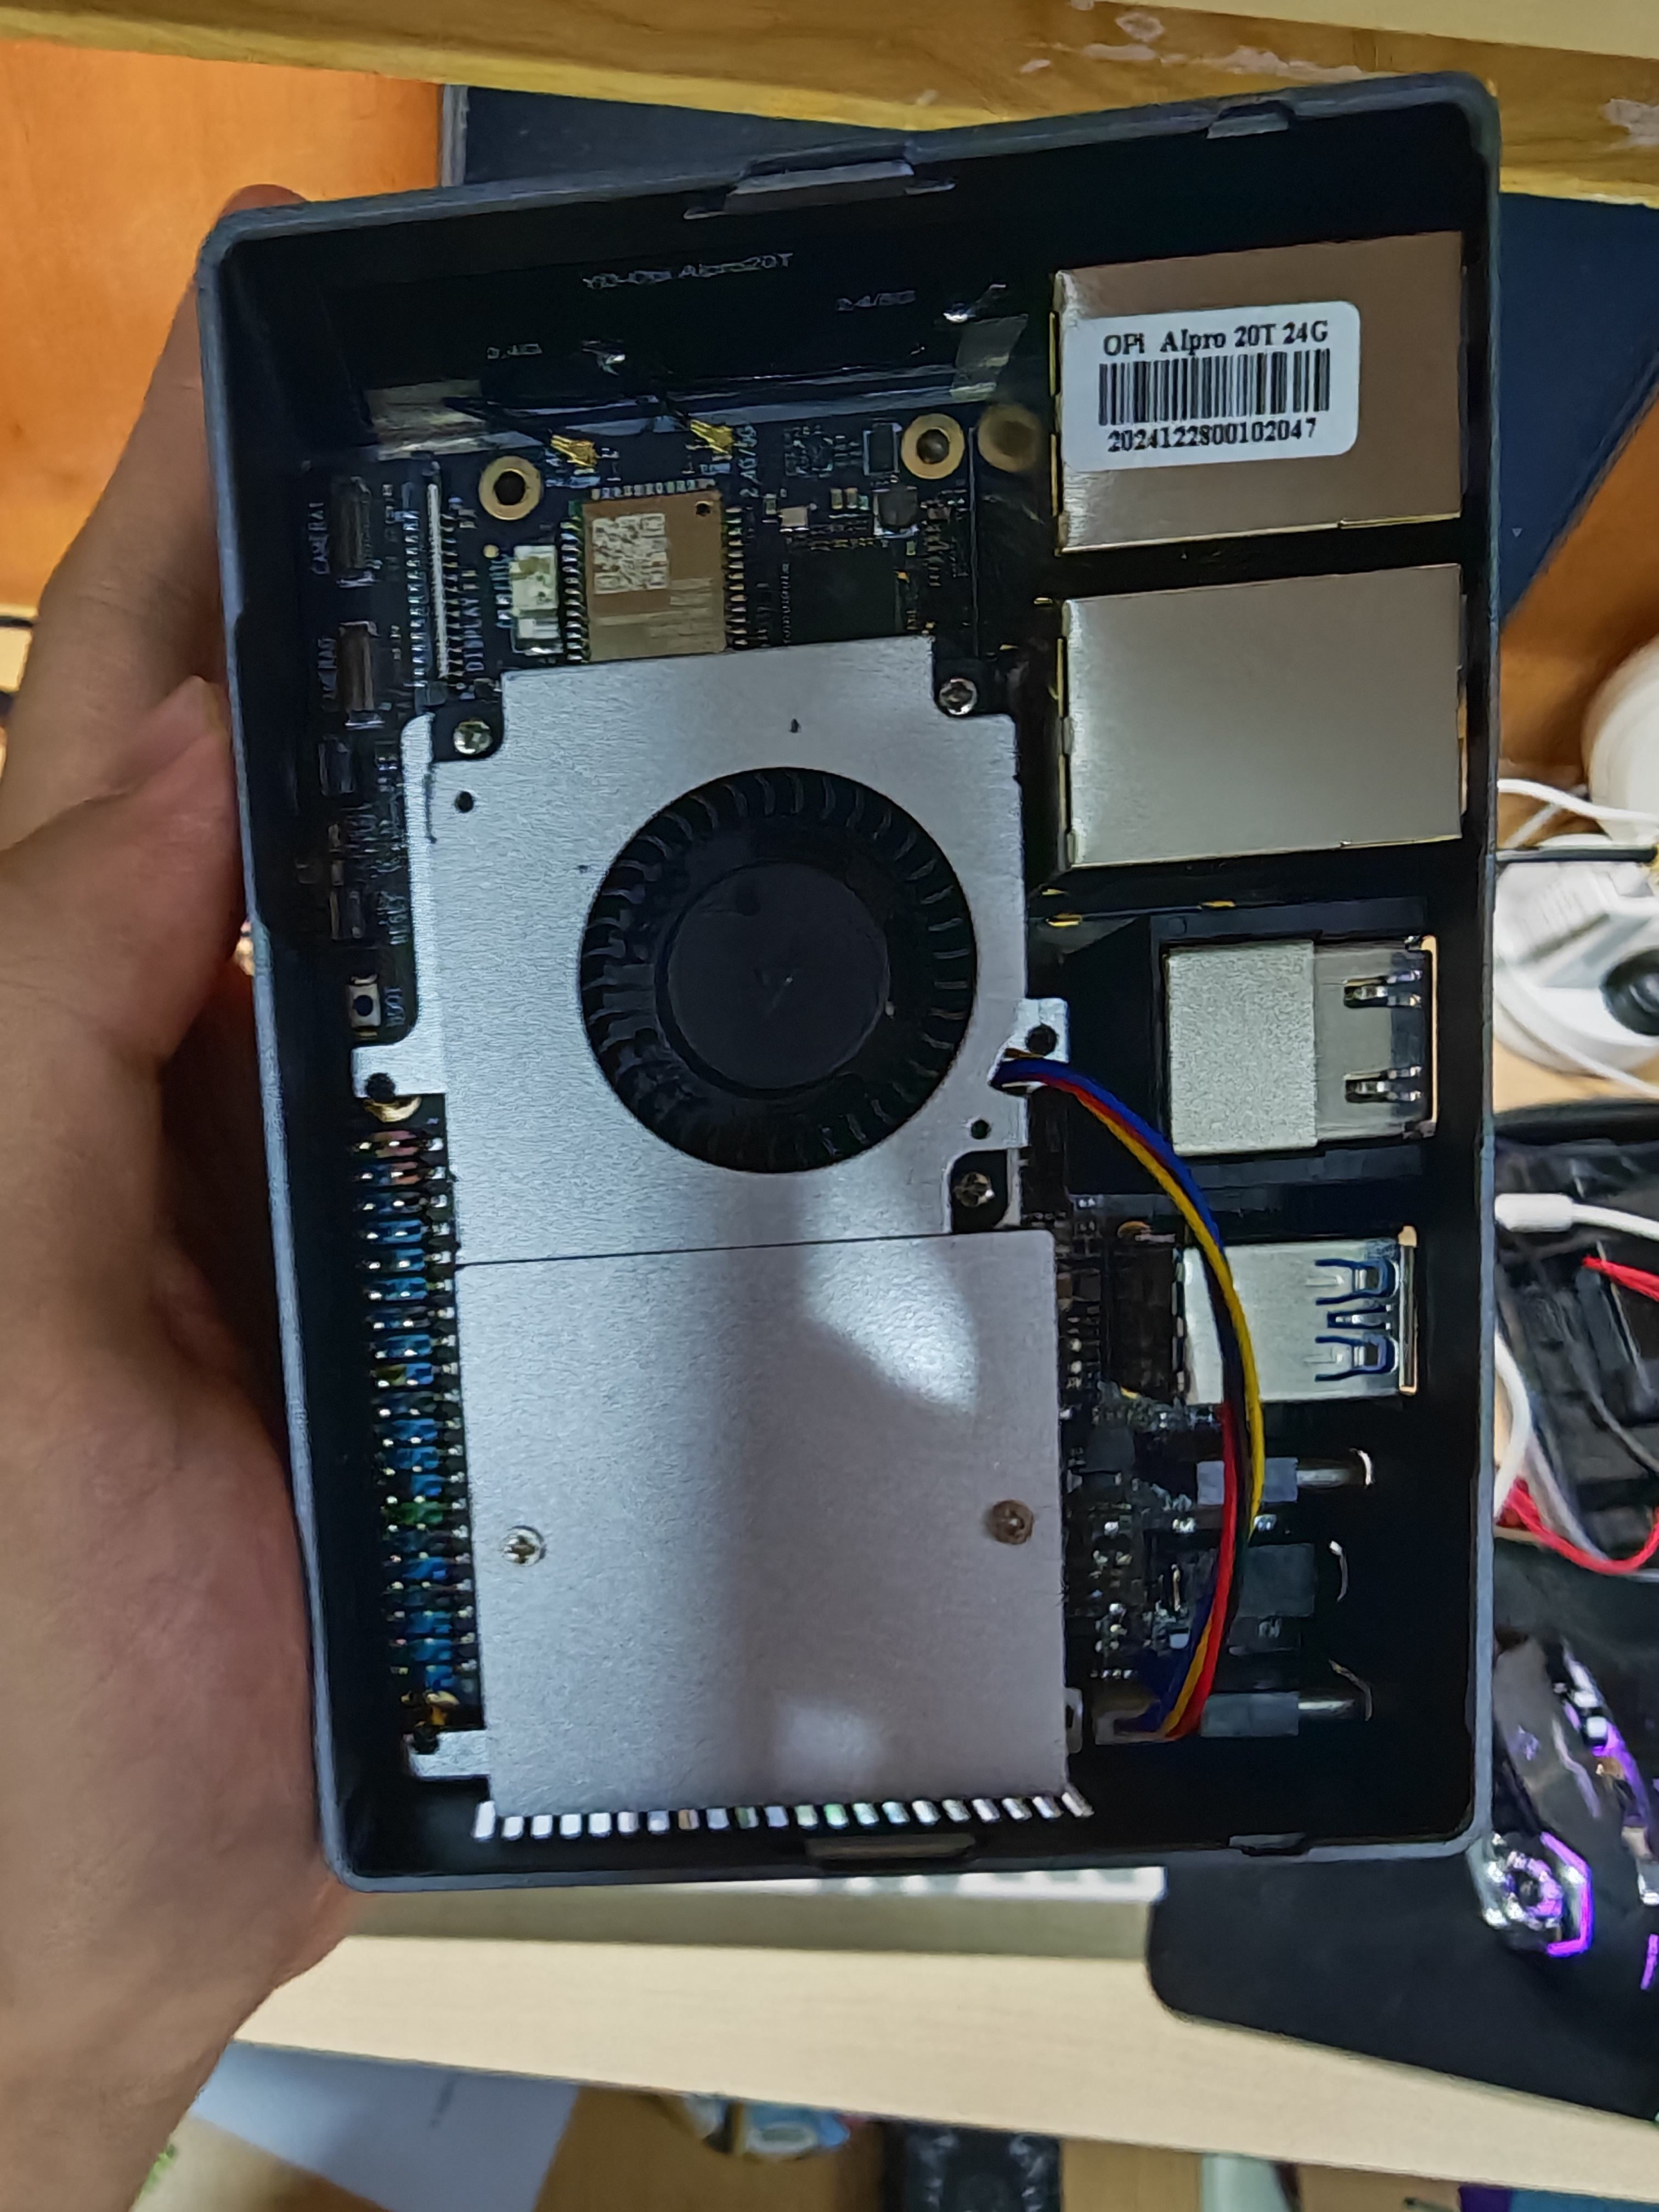
\includegraphics[width=0.8\textwidth]{1.jpg}
    \caption{我的香橙派}
    \label{fig:orangepi}
\end{figure}
\section{markdown学习}
在这一部分,我将记录我在学习Markdown过程中的一些笔记和体会。
\subsection{求是潮的晚安短信}
{\emojifont 📌}第一次尝试用Markdown写文稿(好多内容都是扒下来的哈哈哈哈)

可以直接复制到md编辑器中查看效果
    \begin{lstlisting}[style=markdownstyle]
    # 🌙 清风的晚安短信

> **惟江上之清风,与山间之明月**
> **愿你我不负时光,愿时光不负相遇**
---
## 👤 关于我
- **身份**:25产研小登
- **ID**:清风
- **班级**:工信2524
- **籍贯**:黑龙江哈尔滨
- **性格**:时i时e(自己也搞不清楚,比较乐观吧,很乐意和大家交朋友
- ##### 我的所有账号的ID几乎都是“清风”,主要还是来源于《赤壁赋》里面的那句话,不过也有一点点故事(想听可以戳我🐕)
---
## 🗺️关于我的家乡
### ❄️特色
我来自黑龙江哈尔滨,嗯,就是大家熟悉的(应该熟悉吧)冰雪大世界的发源地(这两年项目特别多,夏天的活动也在逐渐开发,冬天活动更多——除了有点冷)。还记得有一次去里面蹦迪(yes室外蹦迪)特别爽,欢迎大家来玩呀
### 📖高中生活
毕业于哈三中,黑龙江省最好的省重点。我高中的时候成绩还是挺好的…也好几次考过年级前二十;高考前面几个月感觉特别累,主要是北方懂得都懂,管理方面不如南方,所以好多都是自己学(练习册和模拟卷学校发的根本不够做),当时和几个哥们一起卷哈哈哈哈,回想起来也是一段美好的回忆。当时毕业之前老师把我还有另两个我们班经常考前面的同学调坐(据说是为了风水),结果高考我们几个没一个裸分够清北线,我强基没调剂所以也没过,来到浙里。不过现在觉得也没什么遗憾的,能在这里遇到这么好的你们,还说什么呢~

## 💫 兴趣爱好

### 🎌 第五人格!
IdentityV 资深玩家,沉迷其中无法自拔,欢迎各位朋友加我~

> **症状描述**:第五人格,启动!

### 💻 写代码(主要是自己瞎搞)
虽然分流的时候我目标的一志愿不是计科,但这并不妨碍我对写代码很感兴趣()

**something about**:
- 自学过一点点人工智能
- 最近在搞华为昇腾开发板

### 🏓 乒乓球 🏸羽毛球
- **技能描述**:会打乒乓球(会一点点旋转);羽毛球打的一般,但也能玩哈哈哈
- **现实状况**:欢迎伙伴们找我约球!

---

## 📚 大学生活
- 我算是体会到水课上课水到没边,下课小组作业累到飞起的感觉了(主要是心累…
- 马上就迎来工信的分流(说不紧张是假的,不过好在我并不想去卷计科)因为热衷动手实践,加上从高中开始就对电子感兴趣,目前就打算去电科这样?学长有什么好的建议嘛🥹
- 现在感觉学业压力也没那么大,硬课不多,微积分和线代都还行,闲下来就自己搞点别的玩玩。不过说实话这个体测我是真没绷住(引体一个做不了)感觉自己体育锻炼优点疏忽了,周末想多运动运动吧…别一天天都坐着了
- 社团就加了两个,求是潮和AI协会,基本都是技术型的(太菜了我),希望能够多学点知识技能吧,然后安排好时间劳逸结合

---

## 💑 情感经历
嗯,还在进行时(从高中带过来),不过现在异地(她在上海…
感觉学医的好忙,现在每天说话也不多,不过感情还可以,也不知道能不能坚持下去

---

## 🎯小结
希望产研的伙伴们都能在这个学期收获满满(事业友谊双丰收!)

---
## 🌤️ 天气信息

**西湖区** - 轻风,空气优,紫外线弱

**未来天气**:
| 日期 | 温度 | 日期 | 温度 |
|------|------|------|------|
| 10/20 今天 | 14-19°C | 10/24 周五 | 14-21°C |
| 10/21 明天 | 15-17°C | 10/25 周六 | 13-20°C |
| 10/22 周三 | 14-18°C | 10/26 周日 | 13-20°C |
| 10/23 周四 | 14-19°C | 10/27 周一 | 12-20°C |

    \end{lstlisting}
\subsection{求是潮内训}
\subsubsection{后端第一次}
\subsection{e志者协会课}
    \begin{itemize}
        \item 属于我的一台电脑
    \end{itemize}
    
\end{document}